\section{Label-Independent Notions of Symmetry} \label{sec:labindnotions}
\subsection{Notions of Fairness (work in progress)} %\label{subsec:labelindepnotionsoffairness}

\begin{definition}
	We shall refer to a game $\Gamma = (N, A, u)$ as:
	\begin{enumerate}
		\item \textit{strictly fair} if the 
		\item \textit{$n$-transitively strictly fair} if
		\item \textit{ordinally fair} if "there is a transitive subgroup of bijections that preserve preferences over pure strategy profiles" (need to work out how to phrase this);
		\item \textit{$n$-transitively ordinally fair} 
		\item \textit{cardinally fair} if "there is a transitive subgroup of bijections that preserve preferences over mixed strategy profiles". 
		\item \textit{$n$-transitively cardinally fair} if 
	\end{enumerate}
\end{definition}

\subsection{Notions of Symmetry} \label{subsec:labelindepnotionsofsymmetry}
Similar to our label-independent characterisations of our label-dependent notions of anonymity, Theorem \ref{strattrivmatchingthm} gives us the following label-independent characterisations of our label-dependent notions of fairness.

\begin{corollary} \label{indchar1}
	The following conditions are equivalent:
	\begin{enumerate}
		\item There exists standard symmetric $\Gamma'$ such that $\Gamma \cong \Gamma'$;
		\item $\Gamma$ has a player transitive and strategy trivial subgroup $G$; and
		\item There exists a matching $M$ and player transitive $T \leq S_N$ such that $M_{T} \leq \Aut(\Gamma)$.
	\end{enumerate}
\end{corollary}

\begin{corollary}  \label{indchar2}
	The following conditions are equivalent:
	\begin{enumerate}
		\item There exists fully symmetric $\Gamma'$ such that $\Gamma \cong \Gamma'$;
		\item $\Gamma$ has a player $n$-transitive and strategy trivial subgroup $G$; and
		\item There exists a matching $M$ such that $M_{S_N} \leq \Aut(\Gamma)$.
	\end{enumerate}
\end{corollary}

Henceforth we will use fully and standard symmetric to refer to our label-independent characterisations. 

\begin{corollary}
	If $\Gamma$ is standard symmetric then there exists a matching $M$ such that for each $s \in M$, $u_i(s) = u_j(s)$ for all $i, j \in N$.
	\begin{proof}
		This follows from Lemma \ref{matchingfixedpointlemma}.
	\end{proof}
\end{corollary}

Remember that the defining features for standard and fully symmetric games inside our label-dependent framework were that players be indifferent between which position they play and the arrangement of the players respectively. Inside our label-independent framework, these defining features capture larger classes of fair games.

\begin{definition}
	A game is \textit{symmetric} \cite{NoahXE} if its automorphism group is player transitive and \textit{$n$-transitively symmetric} if its automorphism group is player $n$-transitive.
\end{definition}

\begin{example} The automorphism group of Matching Pennies in Example \ref{MPeg} is \begin{align*}
		\Aut(\Gamma) = \langle &\bigl((12) ; \bigl(\begin{smallmatrix} H & T \\ H & T \end{smallmatrix}\bigr), \bigl(\begin{smallmatrix} H & T \\ T & H \end{smallmatrix}\bigr)\bigr)\rangle \\
		= \{ &\bigl(e ; \bigl(\begin{smallmatrix} H & T \\ H & T \end{smallmatrix}\bigr), \bigl(\begin{smallmatrix} H & T \\ H & T \end{smallmatrix}\bigr)\bigr), 
		\bigl(e ; \bigl(\begin{smallmatrix} H & T \\ T & H \end{smallmatrix}\bigr), \bigl(\begin{smallmatrix} H & T \\ T & H \end{smallmatrix}\bigr)\bigr), \\
		&\bigl((12) ; \bigl(\begin{smallmatrix} H & T \\ H & T \end{smallmatrix}\bigr), \bigl(\begin{smallmatrix} H & T \\ T & H \end{smallmatrix}\bigr)\bigr),
		\bigl((12) ; \bigl(\begin{smallmatrix} H & T \\ T & H \end{smallmatrix}\bigr), \bigl(\begin{smallmatrix} H & T \\ H & T \end{smallmatrix}\bigr)\bigr) \}.
	\end{align*}
	Since $\Aut(\Gamma)$ is player transitive, is not strategy trivial and contains no proper transitive subgroups, Matching Pennies is an $n$-transitively non-standard symmetric game.
\end{example}

Peleg et al. \cite{peleg1999canonical} and Sudh\"{o}lter et al. \cite{sudholter2000canonical} define a game to be symmetric if $\Aut(\Gamma)/\Gamma_N \cong S_N$. It follows immediately from Corollary \ref{cosetcor} that this is equivalent to a game being $n$-transitively symmetric, and furthermore that $\Aut(\Gamma)/\Gamma_N$ being isomorphic to some transitive subgroup of $S_N$ is equivalent to a game being symmetric.

We now consider games which have a subgroup $G$ isomorphic to $S_N$ with $G_N = \{\id_{\Gamma}\}$. Fully symmetric games obviously satisfy this condition, Example \ref{egntransstandnonfull} shows that the converse of this is false. Below we show that all games satisfying this condition are $n$-transitively standard symmetric games; the author has been unable to show whether the converse holds.

\begin{proposition} \label{subisoimpliesinter}
	If $\Gamma$ has a subgroup $G$ isomorphic to $S_N$ with $G_N = \{\id_{\Gamma}\}$ then it is $n$-transitively standard symmetric. 
	\begin{proof}
		$n$-transitivity of $\Gamma$ follows from $\overrightarrow{G} = S_N$. Now since each $n$-cycle generates a regular subgroup of $S_N$, the subgroup of $G$ generated by an automorphism whose player permutation is an $n$-cycle is transitive and strategy trivial, hence $\Gamma$ is standard symmetric.
	\end{proof}
\end{proposition}

We end our exploration of symmetry notions with games that have a transitive subgroup $G$ isomorphic to $\overrightarrow{\Gamma}$ with $G_N = \{\id_{\Gamma}\}$. Standard symmetric games obviously satisfy this condition. To look at the converse we consider the argument used in Proposition \ref{subisoimpliesinter}. 

If all transitive subgroups of $S_N$ had regular subgroups then games with a transitive subgroup $G$ isomorphic to $\overrightarrow{\Gamma}$ with $G_N = \{\id_{\Gamma}\}$ would be standard symmetric. However this is not the case, Hulpke \cite{hulpke2005constructing} listed the non-regular minimally transitive permutation subgroups up to degree $30$. The smallest example is $\langle (14) \circ (25), (135) \circ (246)\rangle$ of degree $6$ and order $12$. For more information on how the transitive subgroups are constructed see for example \cite[Algorithm 8.1]{hulpke2016connected}. There is a GAP \cite{GAP4} library for transitive groups by Hulpke with manual \cite{hulpketransgrp}.

We will see in Example \ref{sixplayereg} that games which have a transitive subgroup $G$ isomorphic to $\overrightarrow{\Gamma}$ with $G_N = \{\id_{\Gamma}\}$ need not be standard symmetric. 

\subsection{Fairness Discussion} \label{subsec:fairnessdiscussion}
So far we have considered many notions of symmetry, see Subsections \ref{subsec:labeldepnotionsofsymmetry} and \ref{subsec:labelindepnotionsofsymmetry}, which we have also been referring to as notions of fairness. 

When the author was explaining the similarities between symmetry and fairness in the context of games to James East, James posed the analogy of cake cutting to the author. Among numerous relevant topics within the area of fair division, there are several types of problems that have been studied, for example:
\begin{enumerate}
	\item Fair cake-cutting - dividing a set of divisible and heterogeneous goods. The problem is called fair pie-cutting when the cake is a circle;
	\item Fair chore division - dividing a set of divisible and heterogeneous bads;
	\item Fair item assignment - dividing a set of indivisible and heterogeneous goods; and
	\item Fair resource allocation - dividing a set of divisible and homogeneous goods.
\end{enumerate}

The literature for fair cake-cutting dates back to at least 1948, for example see Steinhaus \cite{Steinhauscakecutting} which begins in the first paragraph by suggesting the custom ``of dividing an object into two equal parts by letting one partner halve it and the other choose his half" was already probably many centuries old. Hundreds of papers on the topic have appeared since, referencing them here would drown out the references more relevant to the bulk of this paper. 

For the point the author wishes to make we need not complicate things with who is cutting/dividing, with who is choosing, or with cakes that have different toppings. Rather than keeping the cake analogy, we equivalently consider dividing a $2$-dimensional shape in to $n \in \mathbb{Z}^+$ colours. 

\begin{definition}
	A \textit{division} of a $2$-dimensional shape in to $n \in \mathbb{Z}^+$ colours is a partition of the shape in to $n$ regions, each region coloured with a unique colour. 
\end{definition}

First let us define automorphisms for a shape division.

\begin{definition}
	An \textit{automorphism} of a shape division in to $n$ colours is any combination of rotating and/or reflecting the divided/coloured shape that leads to the exact same shape with the same division. 
\end{definition}

Note that:
\begin{enumerate}
	\item While we do not require the permuted shape to preserve colours for each region, if one region with colour $X$ is permuted to a region of colour $Y$, all regions with colour $X$ are required to permute to regions of colour $Y$; 
	\item Associated with each automorphism of a shape division is a permutation of the colours;
	\item The identity automorphism is to not rotate or reflect the shape, ie. leave it alone; and
	\item We refer to the automorphism group of a shape division as non-trivial when it does not consist of just the identity automorphism.
\end{enumerate}

\begin{definition}
	We shall refer to the division of a $2$-dimensional shape in to $n \in \mathbb{Z}^+$ colours as:
	\begin{enumerate}
		\item \textit{fair} if each colour/region fills the same area;
		\item \textit{symmetric} if the automorphism group of the shape division is non-trivial; and
		\item \textit{strongly symmetric} if the shape division has an automorphism that is not the identity but does preserve the colours of permuted regions, ie. the associated colour permutation is the identity. 
	\end{enumerate}
\end{definition}

Note that all strongly symmetric shape divisions are symmetric. Most people would agree that our definitions for fair and (strongly) symmetric in the context of shape divisions are fairly reasonable, for example:
\begin{enumerate}
	\item Our definition of symmetric covers when the colours are not really relevant, merely help to distinguish between the different regions of the division; and
	\item Our definition of strongly symmetric covers when the colours are important and we want automorphisms to preserve the colour of regions.
\end{enumerate}

It is not difficult to find examples which establish that neither fair nor (strongly) symmetric implies the other when dividing shapes in to colours, see for example Figure \ref{fig:cakecuts}.

\begin{figure}[!ht]
	\begin{center}
		\begin{tikzpicture}
			\draw[thick] (-7,4)--(-7,0)--(-1,0)--(-1,4)--(-7,4);
			\draw[thick] (-6,4)--(-6,0);
			\draw[thick] (-2,4)--(-2,0);
			\fill[pattern=north west lines]  (-7,4)--(-7,0)--(-6,0)--(-6,4);
			\fill[pattern=north west lines]  (-2,4)--(-2,0)--(-1,0)--(-1,4);
			\draw[<->,thick] (-7,4.25)--(-6,4.25);
			\node () at (-6.5,4.5) {$x$};
			\draw[<->,thick] (-6,4.25)--(-2,4.25);
			\node () at (-4,4.5) {$4x$};
			\draw[<->,thick] (-2,4.25)--(-1,4.25);
			\node () at (-1.5,4.5) {$x$};
			
			\draw[thick] (7,4)--(7,0)--(1,0)--(1,4)--(7,4);
			\draw[thick] (2.5,4)--(2.5,0);
			\draw[thick] (4,4)--(4,2);
			\draw[thick] (4,2)--(7,2);
			\fill[pattern=north west lines]  (7,4)--(7,2)--(4,2)--(4,4);
			\fill[pattern=north west lines]  (2.5,4)--(2.5,0)--(1,0)--(1,4);
			\draw[<->,thick] (7,4.25)--(4,4.25);
			\node () at (5.5,4.5) {$2x$};
			\draw[<->,thick] (4,4.25)--(2.5,4.25);
			\node () at (3.25,4.5) {$x$};
			\draw[<->,thick] (2.5,4.25)--(1,4.25);
			\node () at (1.75,4.5) {$x$};
			\draw[<->,thick] (7.25,4)--(7.25,2);
			\node () at (7.5,3) {$y$};
			\draw[<->,thick] (7.25,2)--(7.25,0	);
			\node () at (7.5,1) {$y$};
		\end{tikzpicture}
		\caption{Dividing a rectangle in to two colours/shades such that it is: (strongly) symmetric while not fair (left); and fair while not (strongly) symmetric (right).}
		\label{fig:cakecuts}
		\vspace{-0.5cm}
	\end{center}
\end{figure}	

Note that even if the rectangles from Figure \ref{fig:cakecuts} are squares, we still have that neither fair nor (strongly) symmetric implies the other. It is fairly easy to generalise the examples in Figure \ref{fig:cakecuts} with the same results for dividing a rectangle, including the case of a square, in to $n > 2$ colours. Hence, in the context of shape division, the terms fair and symmetric are far from being equivalent, and hence definitely should not be considered synonymous, to one another. A philosophical discussion could be had on whether two precisely defined terms could and/or should be considered synonymous if they are equivalent in the sense of capturing precisely the same objects.

It could be an interesting direction of research to see where fairness and (strong) symmetry do and do not overlap when dividing various different shapes into various numbers of colours. Nevertheless, it seems reasonable at this point to suggest that in a general context we should not treat the terms fair and symmetric as equivalent or synonymous to one another, as we have just seen two reasonable examples where that would break down.

Without further examination or further discussion this may leave one doubting whether notions of symmetry for games should be referred to as notions of fairness. However, astute readers may have noticed that there are some fundamental differences between our notions of symmetry for shape division compared to our notions of symmetry for games. Our symmetry notions for games have required at the very least that players be indifferent between rearrangements of positions for some transitive subgroup of the player or game permutations. Whereas:
\begin{enumerate}
	\item symmetric in the context of shape division is analogous to defining a game as symmetric if the game has an automorphism not equal to the identity; and
	\item strongly symmetric in the context of shape division is analogous to defining a game as strongly symmetric if the game has an automorphism not equal to the identity but that does use the identity player pemutation.
\end{enumerate}

Neither of these have been considered notions of symmetry for games in this paper, or really anywhere in the literature, with the exception of \cite{ViglizzoarXiv} who define partial symmetries in games for when some players are indifferent between various positions in a game, but not indifferent between all positions. 

The notions of symmetry for games that we have considered would be closer to the following notions of symmetry for dividing shapes. 

\begin{definition}
	We shall refer to the division of a $2$-dimensional shape in to $n \in \mathbb{Z}^+$ colours as:
	\begin{enumerate}
		\item \textit{transitively symmetric} if every colour permutation in a transitive subgroup of all colour permutations is associated to at least one automorphism of the shape division; and
		\item \textit{$n$-transitively symmetric} if every colour permutation is associated to at least one automorphism of the shape division.
	\end{enumerate}
\end{definition}

Note all $n$-transitively symmetric shape divisions are transitively symmetric, and all transitively symmetric cake divisions are:
\begin{enumerate}
	\item fair;
	\item symmetric; and
	\item not necessarily strongly symmetric;
\end{enumerate}

Since both all $n$-transitively symmetric shape divisions and all transitively symmetric shape divisions are fair, it is reasonable to refer to these as notions of fairness for dividing shapes. 

Note the example on the right in Figure \ref{fig:cakecuts} is fair and neither transitively or $n$-transitively symmetric. What does this mean? (obviously fairness isn't captured by transitively or $n$-transitively symmetric, what about for games? Is fairness captured by a game being (transitively) symmetric? Maybe that should lead on to the zero sum discussion? Which might dictate how fairness is discussed prior in the paper, and will probably/likely dictate the next paragraph).

Now consider the notion of fairness for games that players be indifferent between which position they play. What is meant by players being indifferent between which position they play? In the case of zero-sum games, it is common to define fairness based on the (expected/minimax).

Recall from Section \ref{sec:intro} that the term fair has appeared in the context of zero-sum games, noting that zero-sum games are a subclass of strategic-form games. For example a $2$-player zero-sum game is defined as fair when the (minimax or expected) value of the game is $0$, ie. when the expected payoff under perfect play for both players is $0$. This gives us another notion for zero-sum games of players being indifferent between which position they play. 

A $2$-player zero-sum game can be fair without both players having the same number of strategies, so clearly a $2$-player zero-sum game being fair does not imply that it satisfies any of the notions of symmetry defined in this paper. Nor does it really seem to make much sense to refer to a fair $2$-player zero-sum game as symmetric. 

\begin{theorem}
	If a two person zero-sum game $\Gamma$ is symmetric then it is fair (as mentioned earlier, this result is also in von Neumann and Morgenstern \cite[Pages 165-166]{VNM}).
	\begin{proof}
		Let $\pi = (12)$. It follows from $\pi \in \Aut(\Gamma)$ that:
		
		 $\displaystyle\min_{s_2}\max_{s_1}u_1(s_1, s_2) = \min_{s_2}\max_{s_1}u_{\pi(1)}(s_{\pi^{-1}(1)}, s_{\pi^{-1}(2)}) = \min_{s_2}\max_{s_1}u_2(s_2, s_1) = \min_{s_1}\max_{s_2}u_2(s_1, s_2)$.
	\end{proof}
\end{theorem}

%which is both the smallest payoff the minimising player can ensure the maximising player can obtain and the largest payoff the maximising player can ensure the minimising player can obtain.

\begin{enumerate}
	\item Does there exist fair $2$-player $m$-strategy zero-sum games that are not symmetric?
	\item What happens if we define a game as fair if both players have the same minimax and maximin values? 
	\item Does there exist non-zero sum games where all players have minimax=maximin=0? Should these be considered fair?
	\item What about when minimax = same for all players and maximin = same for all players? zero-sum and more generally?
	\item What about when minimax = maximin = same for all players? 
\end{enumerate}

One of our notions of fairness for games is that players be indifferent between which position they play. Game isomorphisms establish that players are indifferent between playing the mapped positions for each game, in the case of game automorphisms we get players being indifferent between playing different positions in the same game. If the automorphism group of a game is player transitive, the players are indifferent between which position they play, consequently any notion of symmetry requiring the automorphism group be player transitive falls inside the notion of fairness that players be indifferent between which position they play. 

Note however that the players may still care about the order/arrangement/positions of their opponents, which is the stronger notion of fairness for games that we have considered. Recall that players are indifferent between the order/arrangement/positions of their opponents when the automorphism group is player $n$-transitive.  

Discuss utility and notions of fairness for shape division.
Discuss game isomorphisms/automorphisms. 
Mention AI! 

This leads us to questions like:
\begin{enumerate}
	\item Are various definitions/notions of fair and symmetric equivalent/synonymous in the context of games?;
	\item If they are not, are there cases where fair or symmetric implies the other?
	\item Should we be using the term fair in the context of symmetric games? 
\end{enumerate}

Roadmap:
\begin{enumerate}
	\item von Neumann's definition of fair for zero-sum games works for all simultaneous-form games;
	\item symmetric games are fair in the above sense (von neumann noted for the n-transitive symmetric case);
	\item not all fair games are symmetric, so none of our notions of symmetric are equivalent to the above sense of fair;
	\item would be good to check which types of symmetric games can be von neumann fair with examples for each possible combination, and find all the parameterised ones up to isomorphism, and count the number of strategically inequivalent games for each parameterised game, so getting the number of games for each symmetry notion up to ismorphism as well etc.
	\item can generalise above sense of fair by requiring players have same maximin values and the same minimax values, and in between by also requiring the maximin values = minimax values;
	\item symmetric games are fair in the sense of both generalisations above;
	\item same as point 3 above because these are weaker senses of fair;
	\item same as point 4 above;
	\item von Neumann's sense of fair does not need to preserve the players' preferences over the (pure/mixed) strategy profiles, ie. does not need to preserve the strategic structure with regards to indifference between positions, so none of our notions of symmetry are captured by the vNM (or weaker) sense of fair (or vice versa);
	\item fair in the sense of players' preferences over the (pure/mixed) strategy profiles is captured with ordinally/cardinally symmetric games (ie. ordinal/cardinal automorphisms are a transitive subgroup of the game bijections/permutations);
	\item would be good to do ordinal/cardinal symmetric games in detail, and see whether we can do much in the way of examples and establishing which combinations are possible (may/should be possible in the cardinal case to argue based off what we learn from normal symmetric game situation);
	\item fair in the sense of players' preferences over the mixed strategy profiles being represented by the exact same utility functions (so payoffs are exactly comparable) is captured by symmetric games (ie. automorphisms are a transitive subgroup of the game bijections/permutations);
	\item hence our notions of symmetry do capture some notions of fairness (including n-transitively symmetric capturing the fairness notion of being indifferent between the positions of their opponents), unlike capturing the vNM (or weaker) notions of fairness, and unlike the first few notions of symmetry for shape divisions capturing our notion of fairness for shape divisions.
\end{enumerate}


\subsection{Classifying A Game} \label{subsec:classifying}
While our distinct symmetry notions give us various descriptive definitions of strategic fairness, they do not give us a constructive way to determine where a particular game lies. We now discuss various strategies for classifying a game which will be crucial later on when identifying examples for each combination of symmetry notions considered in this paper.

The strategies for classifying a game introduced in this subsection are not an attempt to outline all the steps required for algorithms that can be implemented to classify games, though with some gaps filled in many of the strategies could be used in such algorithms. It would be a useful future research direction to examine the complexity of deciding whether a game satisfies each notion of symmetry along with outlining algorithms for classifying a game, a potential application of doing so will be mentioned in Subsection \ref{sec:parameterisedgames}. 

To test whether a game $\Gamma$ is fully or standard symmetric: we first try to construct a matching $M$ of the strategy sets where for each profile $s \in M$, all players have the same payoff. If no such matching exists $\Gamma$ is neither fully nor standard symmetric. For example in Matching Pennies, since there does not exist a strategy profile where all players receive the same payoff, we can conclude Matching Pennies is non-standard symmetric.

If such matchings exist: to test for full symmetry we check whether such a matching induces automorphisms for permutations that generate $S_N$; and to test for standard symmetry we check whether such a matching induces automorphisms for player permutations that generate a transitive subgroup of $S_N$, noting that to conclude non-standard symmetry we must check that the game is not invariant under the bijections induced by any such matching and transitive subgroup of $S_N$. 

The reader should note that every $n$-cycle generates a transitive subgroup of $S_N$, but not all transitive subgroups of $S_N$ contain an $n$-cycle. For example the Klein group $\{e, (12) \circ (34), (13) \circ (24), (14) \circ (23)\}$ is a transitive subgroup of $S_4$ that does not contain any $4$-cycles.

To test for $n$-transitivity we check whether there exists automorphisms for permutations that generate $S_N$; and to test for symmetry (ie. transitivity) we check whether there exists automorphisms for permutations that generate a transitive subgroup of $S_N$, again noting that to conclude that a game is not symmetric we must check that the game is not invariant under any transitive subgroup of $S_{\Gamma}$. 

If we know a game is symmetric (ie. transitive) and want to show it is only-transitive, a sufficient condition is to find a strategy profile $s \in A$ whose payoffs do not appear elsewhere under all possible permutations. For example consider Example \ref{stdsymeg} and suppose it has an automorphism whose player permutation is $(23)$. The payoffs for the profile $(a, a, b)$ are $(3, 7, 4)$, so we would need a strategy profile $s \in A$ with payoffs $(3, 4, 7)$. However no such profile exists, hence Example \ref{stdsymeg} is an only-transitive standard symmetric game.

\subsection{Parameterised Symmetric Games} \label{sec:parameterisedgames}
Given a subset $G$ of game bijections we construct the \textit{parameterised game $\Gamma(G)$ of $G$} as follows: for each $g \in \langle{G}\rangle$, $s \in A$ and $i \in N$, set $u_i(s) = u_{g(i)}\bigl(g(s)\bigr)$. Since automorphisms are closed under composition we have $\langle{G}\rangle \leq \Aut(\Gamma)$, hence each orbit of $(N\times{A})/\langle{G}\rangle$ has the same payoff. An algorithm for this construction method has been implemented by the author in C++, the code is available at \cite{GLCode}.

\begin{example} \label{constructeg}
	Let $G = \{\bigl((12) ; \bigl(\begin{smallmatrix} a & b \\ c & d \end{smallmatrix}\bigr), \bigl(\begin{smallmatrix} c & d \\ a & b \end{smallmatrix}\bigr)\bigr)\}$. For $\Gamma(G)$ we require:
	\begin{align*}
		u_1(a, c) &= u_2(a, c) = \alpha   &   u_1(a, d) &= u_2(b, c) = \gamma \\
		u_1(b, c) &= u_2(a, d) = \beta   &   u_1(b, d) &= u_2(b, d) = \delta
	\end{align*} 
	\begin{center}
	\begin{game}{2}{2}[$\Gamma(G)$]
			  \> $c$  \> $d$ \\
		$a$   \> $\alpha, \alpha $  \> $\gamma, \beta $ \\
		$b$   \> $\beta, \gamma $  \> $\delta, \delta $
	\end{game}
	\end{center}
	
	We call $\alpha, \beta, \gamma, \delta \in \mathbb{R}$ the \textit{parameters} of $\Gamma(G)$. Note that distinct parameter choices may lead to strategically inequivalent games, even though both games will have the same automorphism group. All fully symmetric $2$-player $2$-strategy games are isomorphic to $\Gamma(G)$ for at least one choice of parameters, hence $\Gamma(G)$ is a general form for fully symmetric $2$-player $2$-strategy games, or equivalently standard symmetric $2$-player $2$-strategy games.
\end{example}

	We can define a partial order $\leq$ on parameterised games as follows: $\Gamma(G) \leq \Gamma(G')$ when given a set of parameter choices for $\Gamma(G')$ there exists a set of parameter choices for $\Gamma(G)$ such that $\Gamma(G) \cong \Gamma(G')$. We illustrate our order in Figures \ref{2pHasse} and \ref{3pHasse} using the Hasse diagrams for $\leq$ on parameterised symmetric $2$-player and $3$-player $2$-strategy games up to isomorphism, which were constructed using the code at \cite{GLCode}.

	\begin{figure}[!ht]
		\begin{center}
		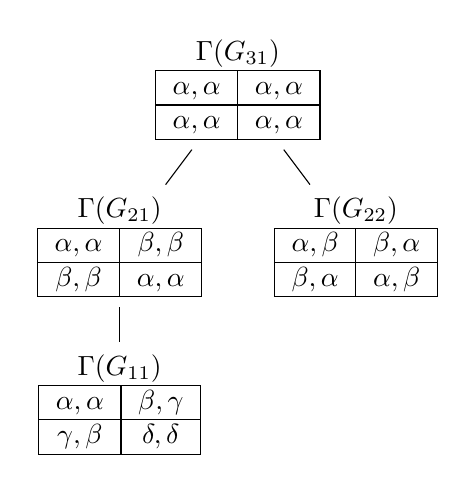
\begin{tikzpicture}
    			\node (r3c1) at (0,0)  {\begin{tabular}{| c | c |}
    			\multicolumn{2}{c}{$\Gamma(G_{31})$}\\
    			\hline
    			$\alpha, \alpha$  & $\alpha, \alpha$ \\ \hline
			$\alpha, \alpha$  & $\alpha, \alpha$ \\
    			\hline
  		\end{tabular}};
	
    			\node (r2c2) at (1.5,-2) {\begin{tabular}{| c | c |}
    			\multicolumn{2}{c}{$\Gamma(G_{22})$}\\
    			\hline
    			$\alpha, \beta$  & $\beta, \alpha$ \\ \hline
			$\beta, \alpha$  & $\alpha, \beta$ \\
    			\hline
  		\end{tabular}};	
	
			\node (r2c1) at (-1.5,-2)  {\begin{tabular}{| c | c |}
    			\multicolumn{2}{c}{$\Gamma(G_{21})$}\\
    			\hline
    			$\alpha, \alpha$  & $\beta, \beta$ \\ \hline
			$\beta, \beta$  & $\alpha, \alpha$ \\
    			\hline
  		\end{tabular}};

			\node (r1c1) at (-1.5,-4)  {\begin{tabular}{| c | c |}
    			\multicolumn{2}{c}{$\Gamma(G_{11})$}\\
    			\hline
    			$\alpha, \alpha$  & $\beta, \gamma$ \\ \hline
			$\gamma, \beta$  & $\delta, \delta$ \\
    			\hline
  		\end{tabular}};
  		
  		\draw (r2c1) -- (r3c1) -- (r2c2);
  		\draw (r2c1) -- (r1c1);
		\end{tikzpicture}
		\end{center}
		
		\begin{center}
		$G_{11} = \{\bigl((12) ; \bigl(\begin{smallmatrix} a & b \\ c & d \end{smallmatrix}\bigr), \bigl(\begin{smallmatrix} c & d \\ a & b \end{smallmatrix}\bigr)\bigr)\}$, $G_{21} = G_{11} \cup \{\bigl((12) ; \bigl(\begin{smallmatrix} a & b \\ d & c \end{smallmatrix}\bigr), \bigl(\begin{smallmatrix} c & d \\ b & a \end{smallmatrix}\bigr)\bigr)\}$,
		
		$G_{22} = \{\bigl((12) ; \bigl(\begin{smallmatrix} a & b \\ d & c \end{smallmatrix}\bigr), \bigl(\begin{smallmatrix} c & d \\ a & b \end{smallmatrix}\bigr)\bigr)\}$, $G_{31} = G_{11} \cup G_{22}$.
		\end{center}
		\vspace{-0.5cm}
		\caption{A plot of the graph of the Hasse diagram for $\leq$ on parameterised symmetric $2$-player $2$-strategy games up to isomorphism.}
		\label{2pHasse}
	\end{figure}
	
	One future direction of research would be to compute the Hasse diagrams for all (symmetric) parameterised games up to isomorphism for a fixed number of players and fixed number of strategies, seeing which combinations of player and strategy counts are computationally feasible with modern day hardware and compilers. One can then also get the poset of (symmetric) games up to isomorphism by finding the strategically inequivalent games for each parameterised game. It would be good to come up with a way to allow us to confirm/verify the result from Goforth and Robinson \cite{GoforthRobinson} that there are 144 ordinal equivalence classes for the 2-player 2-strategy games, which should be possible using game bijections, and obtain numbers for the number of (parameterised) (symmetric) games up to isomorphism for various player and strategy counts.
	
	In order to achieve the above research goals, a number of algorithms beyond those at \cite{GLCode} would need to be examined and implemented, including:
	\begin{enumerate}
		\item Implement algorithms to classify a game for each desired symmetry notion, see Subsection \ref{subsec:classifying} for a discussion on this;
		\item Find a precise and accurate definition for isomorphisms between two parameterised games, which is likely more complicated than for non-parameterised games due to the utilities for outcomes/profiles no longer being ordered;
		\item Implement an algorithm to check whether there exists an isomorphism between two parameterised games, ie. check whether two parameterised games are equivalent. This may require iterating through every relabelling of the players and strategies;
		\item Implement an algorithm for the partial-order we defined on parameterised games;
		\item Implement a struct for posets of strategic-form games ordered using the partial-order algorithm; and
		\item Unless the search space can be reduced, iterate through all appropriate subsets/subgroups of the game bijections, constructing the game for each subset/subgroup, checking that it meets the desired properties in the case of symmetric games, checking whether each new constructed game is equivalent to any games already found, and if it not equivalent to any games already found then insert it in to the poset. 
	\end{enumerate}
	
	When the above is successfully achieved, one will also need a way to output the Hasse diagrams in a way that humans can interpret, preferably also outputting the Hasse diagrams as Ti\emph{K}Z code or code for any other {\LaTeX} package.
	
	The author sees little point in constructing the Hasse diagram for non-parameterised games as it will essentially be the same as the Hasse diagram for parameterised games except each parameterised game is replaced with an equivalence class of strategically inequivalent games that essentially have the same automorphism group.
	
	Subsection \ref{subsec:examples} contains examples of games for the remaining combinations of symmetry notions that examples have not already been given for. These examples were constructed using the code at \cite{GLCode} and using the following strategies.
    
	To construct a symmetric game or an $n$-transitively symmetric game we use bijections that generate a player transitive  or player $n$-transitive subgroup respectively. 
	
	To construct an only-transitive symmetric game it is not sufficient to use bijections that generate an only-transitive subgroup, we must construct $\Gamma(G)$ and check that it is only-transitive. This is due to $\langle{G}\rangle$ possibly being a proper subgroup of $\Aut(\Gamma)$. For example, if we take:
	\[G = \{ \bigl((123) ; \bigl(\begin{smallmatrix} a & b \\ d & c \end{smallmatrix}\bigr), \bigl(\begin{smallmatrix} c & d \\ e & f \end{smallmatrix}\bigr), \bigl(\begin{smallmatrix} e & f \\ a & b \end{smallmatrix}\bigr)\bigr),
               \bigl((123) ; \bigl(\begin{smallmatrix} a & b \\ c & d \end{smallmatrix}\bigr), \bigl(\begin{smallmatrix} c & d \\ f & e \end{smallmatrix}\bigr), \bigl(\begin{smallmatrix} e & f \\ a & b \end{smallmatrix}\bigr)\bigr) \},\] 
    then $N\times{A}$ has one orbit under $\langle{G}\rangle$ (i.e. $\Gamma(G)$ has one parameter/payoff) despite $\langle{G}\rangle$ being an only-transitive subgroup.    
        
	To construct a standard symmetric game we use the bijections induced from a matching of the strategy sets and player permutations which generate a transitive subgroup of $S_N$. To construct a non-standard symmetric game, we first choose game bijections which are not obviously from the same matching, construct $\Gamma(G)$ and check whether it is non-standard symmetric. We construct fully and non-fully symmetric games similarly.
	
\subsection{Further examples} \label{subsec:examples}
So far we have seen examples of fully symmetric, only-transitive standard symmetric and $n$-transitively non-standard symmetric games. We now look at examples constructed with the code at \cite{GLCode} to show that our notions of symmetry are related as shown in the Euler diagram in Figure \ref{fig:Eulerdiag}. A similar approach with regards to constructing examples has been taken by the author and East in \cite{EastHam} within the context of lattice path enumeration to give the precise relationships between finiteness properties of path counts to end points, geometrical properties of the underlying step set, algebraic properties of the monoid of end points, and combinatorial properties of a certain bi-labelled digraph naturally associated to the underlying step set. Knowing the precise relationship between the various notions of symmetry is useful for:
\begin{enumerate}
	\item The theory of (symmetric) games and more generally from a pure mathematics perspective; and
	\item Identifying which combinations of symmetry notions may appear in areas like artificial intelligence, biology, computer science, economics, legal systems, logic, philosophy, politics, along with social choice and voting theory. Though a more thorough investigation of examples for each feasible combination would be needed to identify which strategic situations arise in different contexts. 
\end{enumerate}

\begin{figure}[!ht]
	\begin{center}
	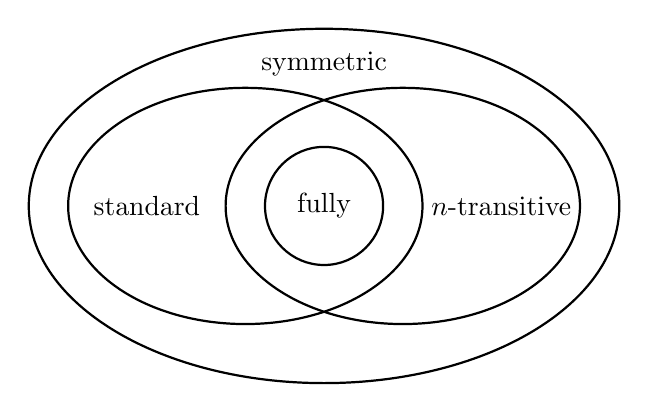
\begin{tikzpicture}
		nodes={draw, ultra thick}
		\draw[thick] (0,0) circle (0.75cm);			\draw (0, 0) node {fully};
		\draw[thick] (-1,0) ellipse (2.25cm and 1.5cm);	\draw (-2.25,0) node {standard};
		\draw[thick] (1,0) ellipse (2.25cm and 1.5cm);	\draw (2.25,0) node {$n$-transitive};
		\draw[thick] (0,0) ellipse (3.75cm and 2.25cm);	\draw (0,1.8) node {symmetric};
	\end{tikzpicture}
	\end{center}
	\vspace{-0.5cm}
	\caption{Euler diagram for label-independent symmetry notions.}
	\label{fig:Eulerdiag}
\end{figure}

\begin{example} \label{egntransstandnonfull}	
	An $n$-transitively non-fully standard symmetric $3$-player game.
	\begin{center}
	\begin{game}{2}{2}[$(a,,)$]
			\>  $e$      \>  $f$      \\
		$c$ \>  $\alpha,\alpha,\alpha$  \>  $\beta,\gamma,\delta$  \\
		$d$ \>  $\gamma,\delta,\beta$  \>  $\delta,\gamma,\beta$  
	\end{game}
	\hspace*{5mm}
	\begin{game}{2}{2}[$(b,,)$]
			\>  $e$      \>  $f$      \\
		$c$ \>  $\delta,\beta,\gamma$  \>  $\beta,\delta,\gamma$  \\
		$d$ \>  $\gamma,\beta,\delta$  \>  $\alpha,\alpha,\alpha$  
	\end{game}
	\end{center}
	
	\begin{align*}
		G = \{\bigl((123) ; \bigl(\begin{smallmatrix} a & b \\ c & d \end{smallmatrix}\bigr), \bigl(\begin{smallmatrix} c & d \\ e & f \end{smallmatrix}\bigr), \bigl(\begin{smallmatrix} e & f \\ a & b \end{smallmatrix}\bigr)\bigr), \bigl((12) ; \bigl(\begin{smallmatrix} a & b \\ d & c \end{smallmatrix}\bigr), \bigl(\begin{smallmatrix} c & d \\ b & a \end{smallmatrix}\bigr), \bigl(\begin{smallmatrix} e & f \\ f & e \end{smallmatrix}\bigr)\bigr)\}
	\end{align*}	

    Since $\langle{G}\rangle$ is $n$-transitive, and the first generator generates a player transitive and strategy trivial group with the matching $M  = \{(a,c,e), (b,d,f)\}$, $\Gamma(G)$ is $n$-transitively and standard symmetric. Furthermore since the bijections induced by $M$ from player transpositions are not automorphisms, $\Gamma(G)$ is non-fully symmetric.
\end{example}

\begin{figure} 
		\begin{center}
		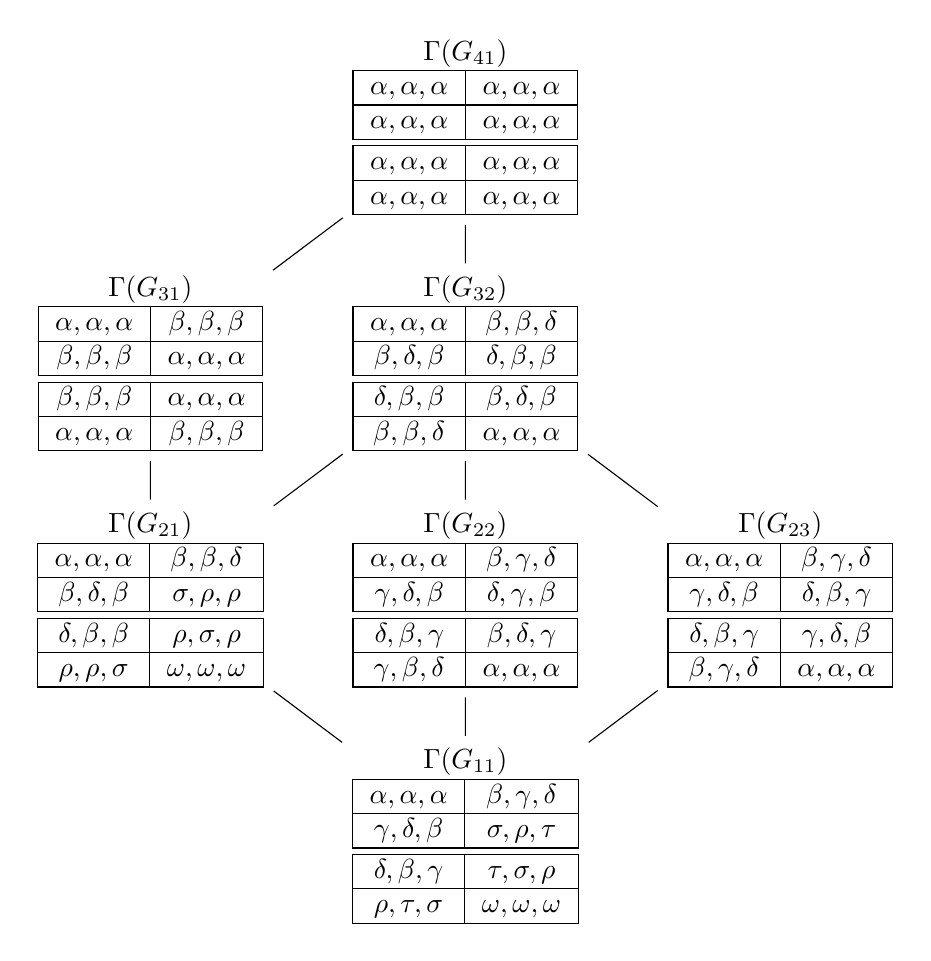
\begin{tikzpicture}
    			\node (r4c1) at (0,0)  {\begin{tabular}{| c | c |}
    			\multicolumn{2}{c}{$\Gamma(G_{41})$}\\
    			\hline
    			$\alpha,\alpha,\alpha$ & $\alpha,\alpha,\alpha$ \\ \hline
				$\alpha,\alpha,\alpha$ & $\alpha,\alpha,\alpha$ \\
    			\hline \hline
				$\alpha,\alpha,\alpha$ & $\alpha,\alpha,\alpha$ \\ \hline
				$\alpha,\alpha,\alpha$ & $\alpha,\alpha,\alpha$ \\
    			\hline
  		\end{tabular}};
			
    			\node (r3c1)  at (-4,-3)    {\begin{tabular}{| c | c |}
    			\multicolumn{2}{c}{$\Gamma(G_{31})$}\\
    			\hline
    			$\alpha,\alpha,\alpha$ & $\beta,\beta,\beta$ \\ \hline
			$\beta,\beta,\beta$ & $\alpha,\alpha,\alpha$ \\
    			\hline \hline
			$\beta,\beta,\beta$ & $\alpha,\alpha,\alpha$ \\ \hline
			$\alpha,\alpha,\alpha$ & $\beta,\beta,\beta$ \\
    			\hline
  		\end{tabular}};
			
			\node (r3c2)  at (0,-3)     {\begin{tabular}{| c | c |}
			\multicolumn{2}{c}{$\Gamma(G_{32})$}\\
    			\hline
    			$\alpha,\alpha,\alpha$ & $\beta,\beta,\delta$ \\ \hline
			$\beta,\delta,\beta$ & $\delta,\beta,\beta$ \\
    			\hline \hline
			$\delta,\beta,\beta$ & $\beta,\delta,\beta$ \\ \hline
			$\beta,\beta,\delta$ & $\alpha,\alpha,\alpha$  \\
    			\hline
  		\end{tabular}};
			
			\node (r2c1)  at (-4,-6)    {\begin{tabular}{| c | c |}
			\multicolumn{2}{c}{$\Gamma(G_{21})$}\\
    			\hline
    			$\alpha,\alpha,\alpha$ & $\beta,\beta,\delta$ \\ \hline
			$\beta,\delta,\beta$ & $\sigma,\rho,\rho$ \\
    			\hline \hline
			$\delta,\beta,\beta$ & $\rho,\sigma,\rho$ \\ \hline
			$\rho,\rho,\sigma$ & $\omega,\omega,\omega$  \\
    			\hline
  		\end{tabular}};
			
			\node (r2c2)  at  (0,-6)    {\begin{tabular}{| c | c |}
			\multicolumn{2}{c}{$\Gamma(G_{22})$}\\
    			\hline
    			$\alpha,\alpha,\alpha$ & $\beta,\gamma,\delta$ \\ \hline
			$\gamma,\delta,\beta$ & $\delta,\gamma,\beta$ \\
    			\hline \hline
			$\delta,\beta,\gamma$ & $\beta,\delta,\gamma$ \\ \hline
			$\gamma,\beta,\delta$ & $\alpha,\alpha,\alpha$  \\
    			\hline
  		\end{tabular}};
			
			\node (r2c3)  at (4,-6)     {\begin{tabular}{| c | c |}
			\multicolumn{2}{c}{$\Gamma(G_{23})$}\\
    			\hline
    			$\alpha,\alpha,\alpha$ & $\beta,\gamma,\delta$ \\ \hline
			$\gamma,\delta,\beta$ & $\delta,\beta,\gamma$ \\
    			\hline \hline
			$\delta,\beta,\gamma$ & $\gamma,\delta,\beta$ \\ \hline
			$\beta,\gamma,\delta$ & $\alpha,\alpha,\alpha$  \\
    			\hline
  		\end{tabular}};	
			
			\node (r1c1)  at (0,-9)     {\begin{tabular}{| c | c |}
			\multicolumn{2}{c}{$\Gamma(G_{11})$}\\
    			\hline
    			$\alpha,\alpha,\alpha$ & $\beta,\gamma,\delta$ \\ \hline
			$\gamma,\delta,\beta$ & $\sigma,\rho,\tau$ \\
    			\hline \hline
			$\delta,\beta,\gamma$ & $\tau,\sigma,\rho$ \\ \hline
			$\rho,\tau,\sigma$ & $\omega,\omega,\omega$  \\
    			\hline
  		\end{tabular}};
  			
  		\draw (r3c1) -- (r4c1) -- (r3c2);
  		\draw (r3c1) -- (r2c1) -- (r3c2) -- (r2c2);
  		\draw (r3c2) -- (r2c3);
  		\draw (r2c1) -- (r1c1) -- (r2c2);
  		\draw (r2c3) -- (r1c1);
			
		\end{tikzpicture}
		\end{center}
		
		\begin{center}
		$G_{11} = \{\bigl((123) ; \bigl(\begin{smallmatrix} a & b \\ c & d \end{smallmatrix}\bigr), \bigl(\begin{smallmatrix} c & d \\ e & f \end{smallmatrix}\bigr), \bigl(\begin{smallmatrix} e & f \\ a & b \end{smallmatrix}\bigr)\bigr)\}$, 
		
		$G_{21} = G_{11} \cup \{\bigl((12) ; \bigl(\begin{smallmatrix} a & b \\ c & d \end{smallmatrix}\bigr), \bigl(\begin{smallmatrix} c & d \\ a & b \end{smallmatrix}\bigr), \bigl(\begin{smallmatrix} e & f \\ e & f \end{smallmatrix}\bigr)\bigr)\}$,
		
		$G_{22} = G_{11} \cup \{\bigl((12) ; \bigl(\begin{smallmatrix} a & b \\ d & c \end{smallmatrix}\bigr), \bigl(\begin{smallmatrix} c & d \\ b & a \end{smallmatrix}\bigr), \bigl(\begin{smallmatrix} e & f \\ f & e \end{smallmatrix}\bigr)\bigr)\}$,
		
		$G_{23} = \{\bigl((123) ; \bigl(\begin{smallmatrix} a & b \\ d & c \end{smallmatrix}\bigr), \bigl(\begin{smallmatrix} c & d \\ f & e \end{smallmatrix}\bigr), \bigl(\begin{smallmatrix} e & f \\ b & a \end{smallmatrix}\bigr)\bigr)\}$,
		
		$G_{31} = G_{21} \cup \{\bigl((123) ; \bigl(\begin{smallmatrix} a & b \\ d & c \end{smallmatrix}\bigr), \bigl(\begin{smallmatrix} c & d \\ f & e \end{smallmatrix}\bigr), \bigl(\begin{smallmatrix} e & f \\ a & b \end{smallmatrix}\bigr)\bigr)\}$,
		
		$G_{32} = G_{2i} \cup G_{2j}$ for all distinct $i, j \in \{1,2,3\}$,
		
		$G_{41} = G_{31} \cup G_{32}$.
		\end{center}
		
		\vspace{-0.5cm}
		\caption{A plot of the graph of the Hasse diagram for $\leq$ on parameterised symmetric $3$-player $2$-strategy games up to isomorphism.}
		\label{3pHasse}
	\end{figure}
	
Cheng et al. \cite{CRVWSym} showed that fully symmetric $2$-strategy games have at least one pure strategy Nash equilibrium. They also noted that Rock, Paper, Scissors is an example of a fully symmetric $2$-player $3$-strategy game with no pure strategy Nash equilibria, and indirectly that Matching Pennies is an example of a non-standard symmetric $2$-player $2$-strategy game which has no pure strategy Nash equilibria. The reader may like to verify that Example \ref{stdsymeg} is a standard symmetric $2$-strategy game with no pure strategy Nash equilibria. 

Note Example \ref{egntransstandnonfull} is the only parameterised $n$-transitively non-fully standard symmetric $3$-player $2$-strategy game up to isomorphism. Furthermore note there are pure strategy Nash equilibria for each choice of parameters. The author has been unable to show whether the result from Cheng et al. \cite{CRVWSym} weakens to $n$-transitively standard symmetric $2$-strategy games.

\begin{example} \label{OTNSeg}
Two only-transitive non-standard symmetric $4$-player games.
\begin{center}
  \begin{game}{2}{2}[$(a,c,,)$]
       \>  $g$          \>  $h$          \\
    $e$  \>  $\alpha,\beta,\gamma,\delta$  \>  $\rho,\tau,\sigma,\omega$  \\
    $f$  \>  $\sigma,\omega,\rho,\tau$  \>  $\omega,\rho,\tau,\sigma$  
  \end{game}
  \hspace*{5mm}
  \begin{game}{2}{2}[$(a,d,,)$]
       \>  $g$          \>  $h$          \\
    $e$  \>  $\delta,\alpha,\beta,\gamma$  \>  $\tau,\sigma,\omega,\rho$  \\
    $f$  \>  $\gamma,\delta,\alpha,\beta$  \>  $\beta,\gamma,\delta,\alpha$  
  \end{game}
  \\
  \begin{game}{2}{2}[$(b,c,,)$]
       \>  $g$          \>  $h$          \\
    $e$  \>  $\beta,\gamma,\delta,\alpha$  \>  $\gamma,\delta,\alpha,\beta$  \\
    $f$  \>  $\tau,\sigma,\omega,\rho$  \>  $\delta,\alpha,\beta,\gamma$  
  \end{game}
  \hspace*{5mm}
  \begin{game}{2}{2}[$(b,d,,)$]
       \>  $g$          \>  $h$          \\
    $e$  \>  $\omega,\rho,\tau,\sigma$  \>  $\sigma,\omega,\rho,\tau$  \\
    $f$  \>  $\rho,\tau,\sigma,\omega$  \>  $\alpha,\beta,\gamma,\delta$  
  \end{game}
\end{center}

\[ G = \{ \bigl((1234) ; \bigl(\begin{smallmatrix} a & b \\ d & c \end{smallmatrix}\bigr), \bigl(\begin{smallmatrix} c & d \\ e & f \end{smallmatrix}\bigr), \bigl(\begin{smallmatrix} e & f \\ g & h \end{smallmatrix}\bigr), \bigl(\begin{smallmatrix} g & h \\ a & b \end{smallmatrix}\bigr)\bigr)\} \]

Since there does not exist any profile where the payoffs are equal and $\langle{G}\rangle$ is transitive, $\Gamma(G)$ is non-standard symmetric. Now for the strategy profile $(a,c,e,g)$ we have payoffs $(\alpha, \beta, \gamma, \delta)$. If $\Gamma(G)$ had an automorphism using $(23)$ then there would be a strategy profile $s \in A$ with payoffs $(\alpha, \gamma, \beta, \delta)$. Since no such profile exists $\Gamma(G)$ is only-transitive.

\begin{center}
  \begin{game}{2}{2}[$(a,c,,)$]
       \>  $g$          \>  $h$          \\
    $e$  \>  $\alpha,\alpha,\beta,\beta$  \>  $\gamma,\delta,\delta,\gamma$  \\
    $f$  \>  $\delta,\gamma,\gamma,\delta$  \>  $\beta,\beta,\alpha,\alpha$  
  \end{game}
  \hspace*{5mm}
  \begin{game}{2}{2}[$(a,d,,)$]
       \>  $g$          \>  $h$          \\
    $e$  \>  $\gamma,\delta,\delta,\gamma$  \>  $\alpha,\alpha,\beta,\beta$  \\
    $f$  \>  $\beta,\beta,\alpha,\alpha$  \>  $\delta,\gamma,\gamma,\delta$  
  \end{game}
  \\
  \begin{game}{2}{2}[$(b,c,,)$]
       \>  $g$          \>  $h$          \\
    $e$  \>  $\delta,\gamma,\gamma,\delta$  \>  $\beta,\beta,\alpha,\alpha$  \\
    $f$  \>  $\alpha,\alpha,\beta,\beta$  \>  $\gamma,\delta,\delta,\gamma$  
  \end{game}
  \hspace*{5mm}
  \begin{game}{2}{2}[$(b,d,,)$]
       \>  $g$          \>  $h$          \\
    $e$  \>  $\beta,\beta,\alpha,\alpha$  \>  $\delta,\gamma,\gamma,\delta$  \\
    $f$  \>  $\gamma,\delta,\delta,\gamma$  \>  $\alpha,\alpha,\beta,\beta$  
  \end{game}
\end{center}

\begin{align*}
G' = \{ \bigl((12) \circ (34) &; \bigl(\begin{smallmatrix} a & b \\ d & c \end{smallmatrix}\bigr), \bigl(\begin{smallmatrix} c & d \\ a & b \end{smallmatrix}\bigr), \bigl(\begin{smallmatrix} e & f \\ h & g \end{smallmatrix}\bigr), \bigl(\begin{smallmatrix} g & h \\ e & f \end{smallmatrix}\bigr)\bigr), \\
               \bigl((13) \circ (24) &; \bigl(\begin{smallmatrix} a & b \\ f & e \end{smallmatrix}\bigr), \bigl(\begin{smallmatrix} c & d \\ h & g \end{smallmatrix}\bigr), \bigl(\begin{smallmatrix} e & f \\ a & b \end{smallmatrix}\bigr), \bigl(\begin{smallmatrix} g & h \\ c & d \end{smallmatrix}\bigr)\bigr), \\
               \bigl((14) \circ (23) &; \bigl(\begin{smallmatrix} a & b \\ h & g \end{smallmatrix}\bigr), \bigl(\begin{smallmatrix} c & d \\ f & e \end{smallmatrix}\bigr), \bigl(\begin{smallmatrix} e & f \\ c & d \end{smallmatrix}\bigr), \bigl(\begin{smallmatrix} g & h \\ a & b \end{smallmatrix}\bigr)\bigr)\}
\end{align*}

That $\Gamma(G')$ is only-transitive non-standard symmetric follows by the same argument used for $\Gamma(G)$. 
\end{example}

\begin{example}
An $n$-transitively non-standard symmetric $4$-player game.
\begin{center}
\begin{game}{2}{2}[$(a,c,,)$]
       \>  $g$          \>  $h$ \\
	$e$  \>  $\alpha,\beta,\beta,\beta$  \>  $\beta,\alpha,\beta,\beta$  \\
    $f$  \>  $\beta,\beta,\beta,\alpha$  \>  $\beta,\beta,\beta,\alpha$  
\end{game}
\hspace*{5mm}
\begin{game}{2}{2}[$(a,d,,)$]
       \>  $g$          \>  $h$          \\
    $e$  \>  $\beta,\beta,\alpha,\beta$  \>  $\beta,\alpha,\beta,\beta$  \\
    $f$  \>  $\beta,\beta,\alpha,\beta$  \>  $\alpha,\beta,\beta,\beta$  
\end{game}
\\
\begin{game}{2}{2}[$(b,c,,)$]
       \>  $g$          \>  $h$          \\
    $e$  \>  $\alpha,\beta,\beta,\beta$  \>  $\beta,\beta,\alpha,\beta$  \\
    $f$  \>  $\beta,\alpha,\beta,\beta$  \>  $\beta,\beta,\alpha,\beta$  
\end{game}
\hspace*{5mm}
\begin{game}{2}{2}[$(b,d,,)$]
       \>  $g$          \>  $h$          \\
    $e$  \>  $\beta,\beta,\beta,\alpha$  \>  $\beta,\beta,\beta,\alpha$  \\
    $f$  \>  $\beta,\alpha,\beta,\beta$  \>  $\alpha,\beta,\beta,\beta$  
\end{game}
\end{center}

\[G = \{ \bigl((1234) ; \bigl(\begin{smallmatrix} a & b \\ c & d \end{smallmatrix}\bigr), \bigl(\begin{smallmatrix} c & d \\ e & f \end{smallmatrix}\bigr), \bigl(\begin{smallmatrix} e & f \\ h & g \end{smallmatrix}\bigr), \bigl(\begin{smallmatrix} g & h \\ a & b \end{smallmatrix}\bigr)\bigr), 
               \bigl((12) ; \bigl(\begin{smallmatrix} a & b \\ c & d \end{smallmatrix}\bigr), \bigl(\begin{smallmatrix} c & d \\ a & b \end{smallmatrix}\bigr), \bigl(\begin{smallmatrix} e & f \\ e & f \end{smallmatrix}\bigr), \bigl(\begin{smallmatrix} g & h \\ h & g \end{smallmatrix}\bigr)\bigr)\}\]

$\Gamma(G)$ is $n$-transitive since $\langle{G}\rangle$ is $n$-transitive, and non-standard symmetric since there does not exist any profile where all players receive the same payoff.
\end{example}

\begin{example} \label{sixplayereg} 
An only-transitive non-standard symmetric $6$-player game that has a subgroup $\langle{G}\rangle$ isomorphic to $\overrightarrow{\langle{G}\rangle}$ with $\langle{G}\rangle_N = \{\id_{\Gamma}\}$.
  
\begin{center}
%\begin{scriptsize}
%\begin{center}
\begin{game}{2}{2}[$(a,c,e,g,,)$]
	\>$k$                 \>$l$  \\
	$i$\>$1,2,1,2,1,2$     \>$3,4,5,6,7,8$\\
	$j$\>$9,10,11,12,13,14$\>$15,16,17,18,19,20$  
\end{game}
\hspace*{5mm}
\begin{game}{2}{2}[$(a,c,e,h,,)$]
	\>$k$                  \>$l$ \\
	$i$\>$5,6,7,8,3,4$      \>$20,15,19,17,18,16$\\
	$j$\>$21,22,23,24,25,26$\>$27,27,28,28,28,27$  
\end{game}
\\
\begin{game}{2}{2}[$(a,c,f,g,,)$]
	\>$k$                  \>$l$ \\
	$i$\>$11,12,13,14,9,10$ \>$29,29,30,30,30,29$\\
	$j$\>$26,24,22,23,21,25$\>$4,8,6,7,5,3$        
\end{game}
\hspace*{5mm}
\begin{game}{2}{2}[$(a,c,f,h,,)$]
	\>$k$                  \>$l$ \\
	$i$\>$17,18,19,20,15,16$\>$8,3,7,5,6,4$\\
	$j$\>$31,32,32,32,31,31$\>$16,20,18,19,17,15$  
\end{game}
\\
\begin{game}{2}{2}[$(a,d,e,g,,)$]
	\>$k$                  \>$l$   \\
	$i$\>$7,8,3,4,5,6$      \>$18,16,20,15,19,17$\\
	j\>$30,29,29,29,30,30$\>$6,4,8,3,7,5$        
\end{game}
\hspace*{5mm}
\begin{game}{2}{2}[$(a,d,e,h,,)$]
	\>$k$                  \>$l$  \\
	$i$\>$19,17,18,16,20,15$\>$32,31,32,31,32,31$\\
	$j$\>$13,11,12,10,14,9$ \>$22,26,24,25,23,21$  
\end{game}
\\
\begin{game}{2}{2}[$(a,d,f,g,,)$]
	\>$k$                  \>$l$   \\
	$i$\>$23,24,25,26,21,22$\>$12,10,14,9,13,11$\\
	$j$\>$14,12,10,11,9,13$ \>$2,2,2,1,1,1$       
\end{game}
\hspace*{5mm}
\begin{game}{2}{2}[$(a,d,f,h,,)$]
	\>$k$                  \>$l$  \\
	$i$\>$28,28,28,27,27,27$\>$24,25,23,21,22,26$\\
	$j$\>$25,23,24,22,26,21$\>$10,14,12,13,11,9$   
\end{game}
\\
\begin{game}{2}{2}[$(b,c,e,g,,)$]
	\>$k$                  \>$l$  \\
	$i$\>$13,14,9,10,11,12$ \>$25,26,21,22,23,24$\\
	$j$\>$21,25,26,24,22,23$\>$31,31,31,32,32,32$  
\end{game}
\hspace*{5mm}
\begin{game}{2}{2}[$(b,c,e,h,,)$]
	\>$k$                  \>$l$  \\
	$i$\>$30,30,30,29,29,29$\>$14,9,13,11,12,10$\\
	$j$\>$9,13,14,12,10,11$ \>$26,21,25,23,24,22$  
\end{game}
\\
\begin{game}{2}{2}[$(b,c,f,g,,)$]
	\>$k$                  \>$l$  \\
	$i$\>$22,23,21,25,26,24$\>$10,11,9,13,14,12$\\
	$j$\>$27,28,27,28,27,28$\>$16,17,15,19,20,18$  
\end{game}
\hspace*{5mm}
\begin{game}{2}{2}[$(b,c,f,h,,)$]
	\>$k$                  \>$l$  \\
	$i$\>$6,7,5,3,4,8$      \>$2,1,1,1,2,2$\\
	$j$\>$15,19,20,18,16,17$\>$4,5,3,7,8,6$  
\end{game}
\\
\begin{game}{2}{2}[$(b,d,e,g,,)$]
	\>$k$                  \>$l$  \\
	$i$\>$19,20,15,16,17,18$\>$28,27,27,27,28,28$\\
	$j$\>$5,3,4,8,6,7$      \>$17,15,16,20,18,19$  
\end{game}
\hspace*{5mm}
\begin{game}{2}{2}[$(b,d,e,h,,)$]
	\>$k$            \>$l$ \\
	$i$\>$7,5,6,4,8,3$\>$23,21,22,26,24,25$\\
	$j$\>$1,1,2,2,2,1$\>$11,9,10,14,12,13$   
\end{game}
\\
\begin{game}{2}{2}[$(b,d,f,g,,)$]
	\>$k$                  \>$l$ \\
	$i$\>$32,32,31,31,31,32$\>$24,22,26,21,25,23$\\
	$j$\>$20,18,16,17,15,19$\>$8,6,4,5,3,7$        
\end{game}
\hspace*{5mm}
\begin{game}{2}{2}[$(b,d,f,h,,)$]
	\>$k$                  \>$l$ \\
	$i$\>$18,19,17,15,16,20$\>$12,13,11,9,10,14$\\
	$j$\>$3,7,8,6,4,5$      \>$29,30,29,30,29,30$  
\end{game}
\\
\vspace{-6mm}
%\end{center}
%\end{scriptsize}
\end{center}

\begin{align*}
G = \{ \bigl((14) \circ (25); &\bigl(\begin{smallmatrix} a & b \\ h & g \end{smallmatrix}\bigr), \bigl(\begin{smallmatrix} c & d \\ i & j \end{smallmatrix}\bigr), \bigl(\begin{smallmatrix} e & f \\ f & e \end{smallmatrix}\bigr), \bigl(\begin{smallmatrix} g & h \\ b & a \end{smallmatrix}\bigr), \bigl(\begin{smallmatrix} i & j \\ c & d \end{smallmatrix}\bigr), \bigl(\begin{smallmatrix} k & l \\ l & k \end{smallmatrix}\bigr)\bigr),\\
               \bigl((135) \circ (246); &\bigl(\begin{smallmatrix} a & b \\ e & f \end{smallmatrix}\bigr), \bigl(\begin{smallmatrix} c & d \\ g & h \end{smallmatrix}\bigr), \bigl(\begin{smallmatrix} e & f \\ i & j \end{smallmatrix}\bigr), \bigl(\begin{smallmatrix} g & h \\ k & l \end{smallmatrix}\bigr), \bigl(\begin{smallmatrix} i & j \\ a & b \end{smallmatrix}\bigr), \bigl(\begin{smallmatrix} k & l \\ c & d \end{smallmatrix}\bigr)\bigr)\}
\end{align*}

Since there does not exist any profile where the payoffs are equal and $\langle{G}\rangle$ is transitive, $\Gamma$ is non-standard symmetric. Now the payoffs for $(a,c,e,g,i,k)$ are $(1, 2, 1, 2, 1, 2)$. If there was an automorphism for $(12)$ then there would be $s \in A$ with payoffs $(2, 1, 1, 2, 1, 2)$. Since no such profile exists $\Gamma$ is only-transitive. It can be verified that $\langle{G}\rangle$ has order $12$, which is equal to the order of $\langle (14) \circ (25), (135) \circ (246)\rangle$, hence $\langle{G}\rangle \cong \langle (14) \circ (25), (135) \circ (246)\rangle$ and $\langle{G}\rangle_N = \{\id_{\Gamma}\}$.
\end{example}

